\chapter{Transmissão em Redes sem Fio}
\label{cap:transmissao-redes-sem-fio}

As ondas de rádio são fáceis de gerar, podem percorrer longas distâncias e penetrar em diversos tipos de materiais, por isso, são amplamente utilizadas para comunicação, desde ambientes abertos até ambientes fechados. As ondas de rádio também são omnidirecionais, o que significa que elas se propagam em todas as direções a partir da origem. Desse modo, o transmissor e o receptor não precisam estar perfeitamente alinhados para que haja comunicação \cite{tanenbaum2011}. Por todas essas características, as ondas de rádio são o principal recurso para que a comunicação sem fio se tornasse possível, resultando em sua dispersão generalizada pelo globo.

\section{O Espectro Eletromagnético}
\label{sec:espectro-eletromagnetico}

Quando se movem, os elétrons criam ondas eletromagnéticas que podem se propagar pelo espaço livre (até mesmo no vácuo), transportando energia durante o percurso. Essas ondas foram previstas pelo físico inglês James Clerk Maxwell em 1865 e foram observadas pela primeira vez pelo físico alemão Heinrich Hertz em 1887 \cite{tanenbaum2011}.

O número de ondas completas que passam por um ponto fixo dentro de um período de tempo é chamado de frequência, e é medido em Hertz (Hz, em homenagem a Heinrich Hertz). A distância entre dois pontos máximos (ou mínimos) consecutivos é chamada comprimento de onda, designada universalmente pela letra grega $\lambda$ (lambda). A \autoref{fig:onda} ilustra essa propriedade das ondas.

A velocidade de uma onda qualquer depende do meio em que ela se propaga. No vácuo, todas as ondas eletromagnéticas viajam na mesma velocidade, a da luz, que é aproximadamente igual a $3 \times 10^8$ m/s, independentemente de sua frequência \cite{tanenbaum2011}.

Essas três grandezas -- frequência ($f$), comprimento de onda ($\lambda$) e velocidade ($c$) -- se relacionam (no vácuo) através da seguinte expressão:

\begin{equation}
	\begin{aligned}
		c = \lambda f
	\end{aligned}
\end{equation}

Desta forma, pode-se observar que as propriedades de uma onda eletromagnética dependem de sua frequência (ou comprimento de onda), já que a velocidade da luz é uma constante.

\begin{figure}[H]
	\centering
	\Caption{\label{fig:onda}Propriedades de uma onda.}	
	\UECEfig{}{
		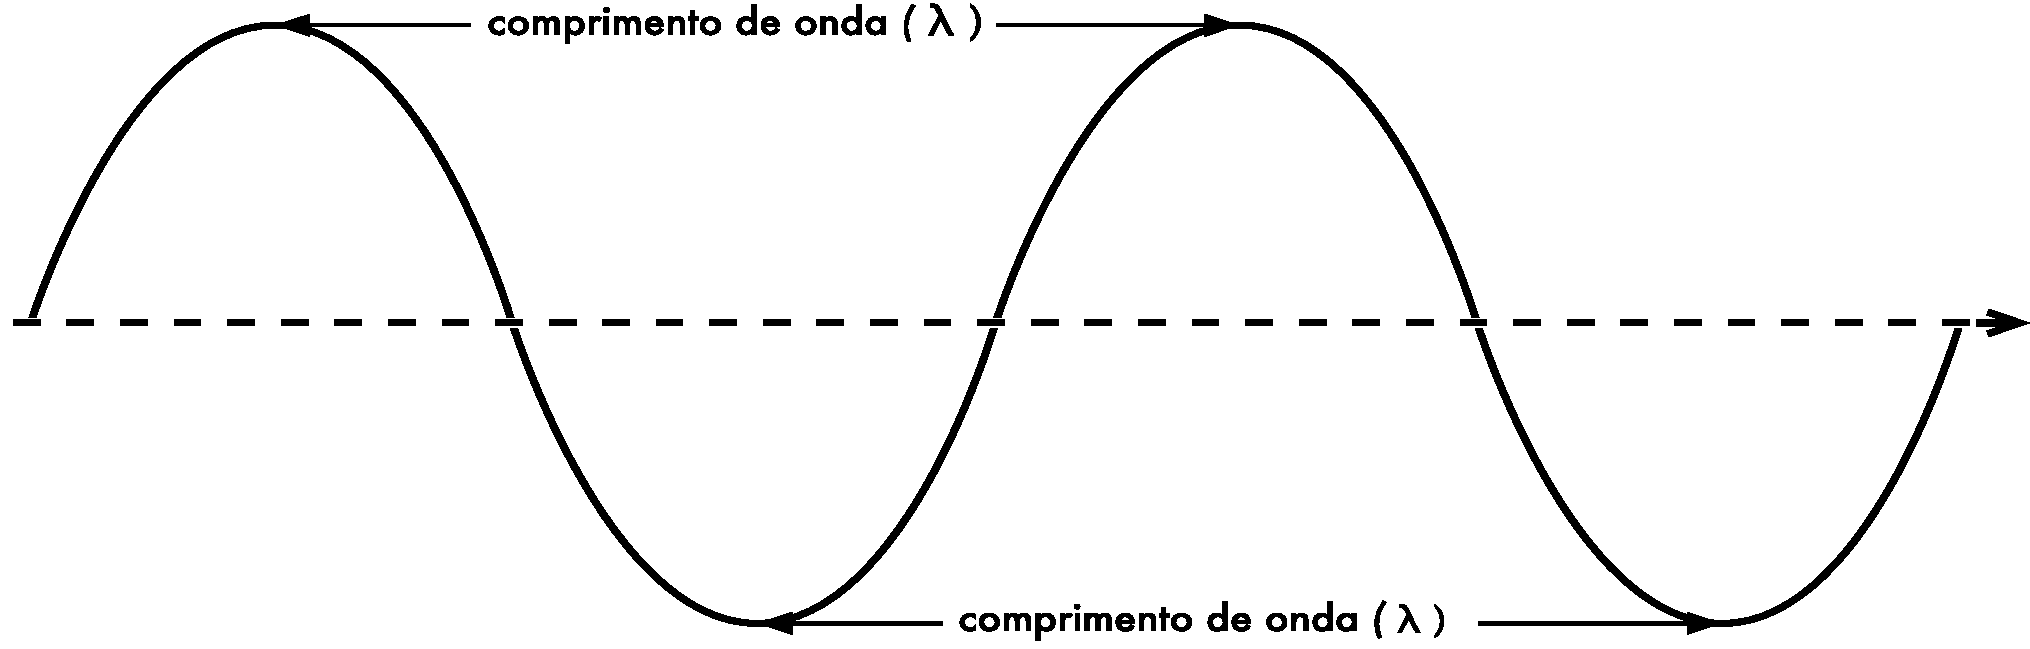
\includegraphics[scale=.4]{figuras/onda_wave.pdf}
	}{
		\Fonte{\citeonline[p. ~10]{flickenger2008}.}
	}	
\end{figure}

Uma onda eletromagnética pode ser gerada ou captada por circuitos eletrônicos simples. Além disso, esse tipo de onda se propaga no vácuo, o que permite a comunicação entre antenas terrestres com satélites no espaço e vice-versa, entre os próprios satélites e entre dois pontos localizados em qualquer parte da superfície terrestre \cite{fluminense2010}.

Os dispositivos sem fio usam ondas eletromagnéticas para transmitir suas informações, porém são restritos para operar em uma determinada banda (ou faixa) de frequência. Cada faixa tem uma largura de banda associada, que é simplesmente a quantidade de espaço de frequência na banda. Se a variação entre 2,40 GHz e 2,48 GHz é usada por um dispositivo, então a largura de banda será de 0,08 GHz ou 80 MHz.

A largura de banda adquiriu uma conotação de ser uma medida da capacidade de dados de um \textit{link}. Uma grande quantidade de matemática, teoria da informação e processamento de sinais pode ser usada para demonstrar que fatias mais largas de frequência podem ser usadas para transmitir mais informações \cite{gast2002}. Por exemplo, um canal de telefonia móvel analógico requer uma largura de banda de 20 kHz. Os sinais de televisão são muito mais complexos, já que, necessariamente, transmitem tráfego de áudio e vídeo, e por esse motivo possuem uma largura de banda consideravelmente maior, cerca de 6 MHz \cite{gast2002}.

Cada banda de frequência utilizada nas telecomunicações estão contidas em um modelo de escala comum, onde é apresentado o intervalo completo de todas as possíveis frequências da radiação eletromagnética, denominado de espectro eletromagnético. A \autoref{fig:espectro} ilustra todas as variações de frequências contidas no espectro eletromagnético.

\begin{figure}[H]
	\centering
	\Caption{\label{fig:espectro}O espectro eletromagnético e a maneira como ele é usado na comunicação.}	
	\UECEfig{}{
		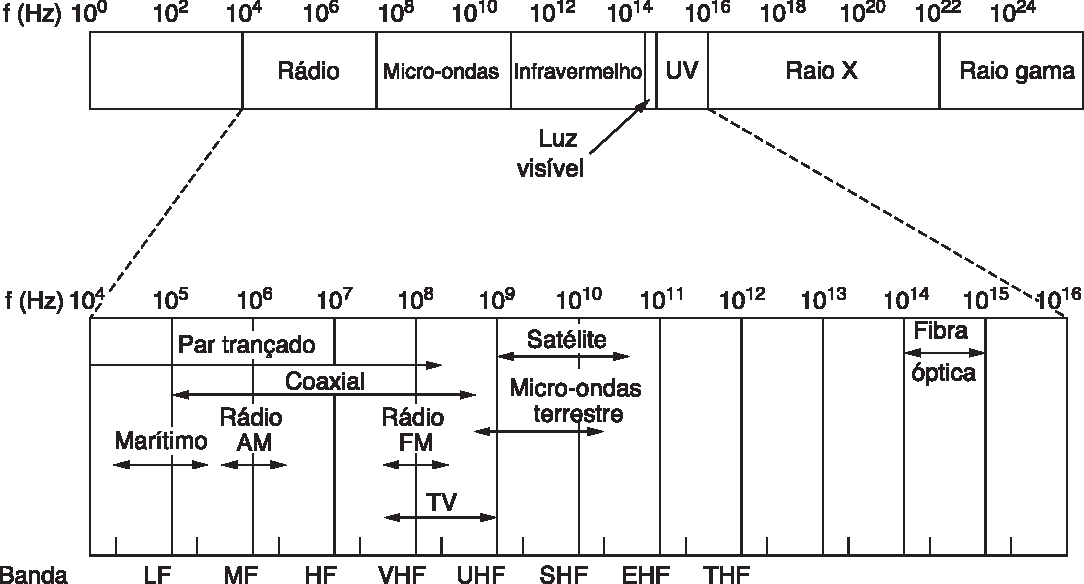
\includegraphics[scale=1]{figuras/espectro_eletromagnetico.pdf}
	}{
		\Fonte{\citeonline[p. ~70]{tanenbaum2011}.}
	}	
\end{figure}

\begin{citacao}
	As faixas de rádio, microondas, infravermelho e luz visível do espectro podem ser usadas na transmissão de informações, por meio de modulação da amplitude, da frequência ou da fase das ondas. A luz ultravioleta, os raios X e os raios gama representariam opções ainda melhores, por terem frequências mais altas, mas são difíceis de produzir e modular, além de não se propagarem bem através dos prédios e de serem perigosos para os seres vivos \cite[p.~65]{tanenbaum2011}.
\end{citacao}

O uso de uma faixa de frequência é rigorosamente controlado pelas autoridades reguladoras através de processos de licenciamento. No âmbito mundial, o processo de padronização de alocação de frequências para uso específico é realizado pela União Internacional de Telecomunicações (ITU, do inglês, \textit{International Telecommunication Union}). No Brasil, a ANATEL (Agência Nacional de Telecomunicações) representa a entidade responsável pela definição e fiscalização da utilização das faixas de frequência em território nacional. Essas determinações regulatórias visam coibir o uso das faixas de frequência sem permissão por infratores como estações de rádio e TVs piratas.

Entretanto, existem faixas de frequência que não estão sujeitas a autorização de uso pelos órgãos reguladores, ou seja, são bandas de frequência abertas para transmitir. Essas frequências não licenciadas são conhecidas como ISM (do inglês, \textit{Industrial, Scientific, Medical}). As bandas ISM foram padronizadas na maioria dos países em três faixas de frequência: 900 MHz, 2.4 GHz e 5 GHz \cite{moraes2010,tanenbaum2011}. A \autoref{fig:ism_unii} exibe a alocação das frequências ISM e também das bandas U-NII (do inglês, \textit{Unlicensed National Information Infrastructure}).

\begin{figure}[H]
	\centering
	\Caption{\label{fig:ism_unii}As bandas ISM e U-NII.}	
	\UECEfig{}{
		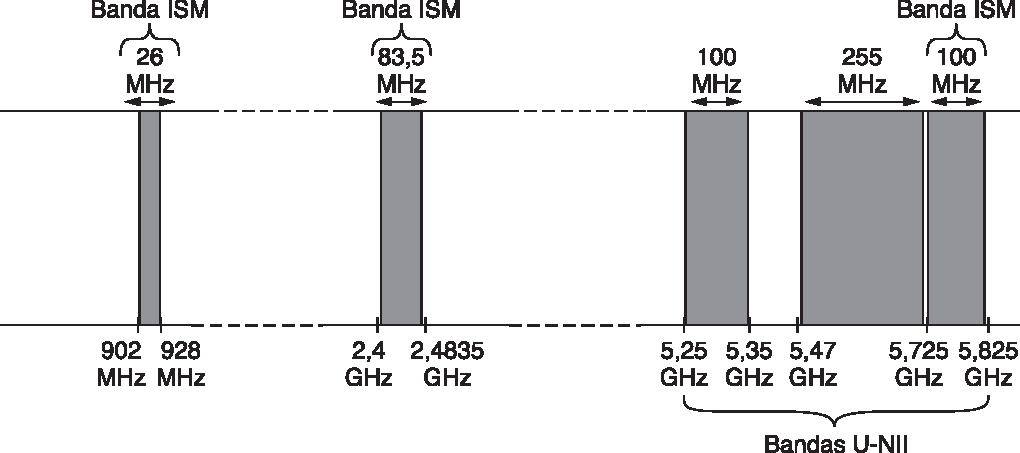
\includegraphics[scale=.64]{figuras/ism-unii.pdf}
	}{
		\Fonte{\citeonline[p. ~66]{tanenbaum2011}.}
	}	
\end{figure}

\section{Efeitos de Propagação em Ondas Eletromagnéticas}
\label{sec:efeitos-propagacao-OE}

Sistemas de comunicações sem fio utilizam-se de ondas eletromagnéticas para o envio de sinais através do ar. Na perspectiva de um usuário, conexões sem fio não são particularmente diferentes de qualquer outro tipo de conexão de rede: os serviços de transmissão de informações funcionarão de acordo com o esperado \cite{flickenger2008}. Mas ondas de rádio possuem algumas propriedades inesperadas se comparadas com o meio guiado.  Por exemplo: é muito fácil ver o caminho que o cabo Ethernet faz, só é preciso seguí-lo em sua extensão. Também pode-se ter a confiança de que ter vários cabos Ethernet lado a lado não causarão problemas, uma vez que os sinais trafegam no interior dos fios.

Diferentemente dos enlaces físicos, o caminho de uma onda de rádio entre transmissor e receptor pode variar de uma simples linha de visão completamente desobstruída até um cenário em que seja obstruído por prédios, terrenos elevados e áreas de vegetação densa \cite{rappaport2009}. Isso quer dizer que os sinais de rádio são aleatórios e de difícil análise. Até a velocidade do deslocamento dos terminais influencia na rapidez com que o sinal enfraquece \cite{rappaport2009}.

Portanto, o estudo da propagação dos sinais de radiofrequência é importante para a compreensão das comunicações sem fio porque fornece a modelagem física necessária, o que resulta em uma boa estimativa de potência requerida para o estabelecimento do enlace de comunicação para que haja comunicação confiável \cite{haykin2008}. Além disso, o estudo da propagação auxilia na compreensão das técnicas de recepção para compensação das perdas introduzidas pela transmissão sem fio \cite{haykin2008}.

Os efeitos sofridos pela onda eletromagnética ao se propagar são diversos, mas os principais são a absorção, a reflexão, a difração, a refração, o desvanecimento e a interferência \cite{flickenger2008,haykin2008,rappaport2009}.

\subsection{Absorção}
\label{sub:absorcao}

Quando ondas eletromagnéticas penetram algum objeto, elas geralmente atenuam ou dissipam-se totalmente, como ilustra a \autoref{fig:absorcao}. O quanto elas perdem de potência irá depender de sua frequência e do material em que penetram \cite{flickenger2008}.

\begin{figure}[H]
	\centering
	\Caption{\label{fig:absorcao}Atenuação de uma onda devido a absorção.}	
	\UECEfig{}{
		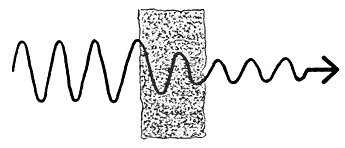
\includegraphics[scale=.75]{figuras/absorcao1.png}
	}{
		\Fonte{Adaptado de \citeonline{megasorber2019c}.}
	}
\end{figure}

Para ondas de rádio, os dois principais materiais absorventes são \cite{flickenger2008}:

\begin{compactitem}
	\item metais: elétrons podem mover-se livremente em metais, sendo prontamente capazes de oscilar e absorver a energia de uma onda que incida sobre eles.
	\item água: ondas de rádio fazem com que as moléculas de água agitem-se, tomando parte da energia da onda.
\end{compactitem}

\subsection{Reflexão}
\label{sub:reflexao}

Nas comunicações sem fio terrestres, normalmente não existe uma linha de visada desimpedida no percurso do sinal de rádio entre transmissor e receptor e as comunicações geralmente envolvem o fenômeno da reflexão \cite{haykin2008}. O fenômeno da reflexão de ondas eletromagnéticas é mostrado na \autoref{fig:reflexao}.

``A reflexão ocorre quando uma onda eletromagnética em propagação colide com um objeto que possui dimensões muito grandes em comparação com o comprimento de onda da onda que se propaga'' \cite[p.~76]{rappaport2009}.

\begin{figure}[H]
	\centering
	\Caption{\label{fig:reflexao}Reflexão de ondas de rádio.}	
	\UECEfig{}{
		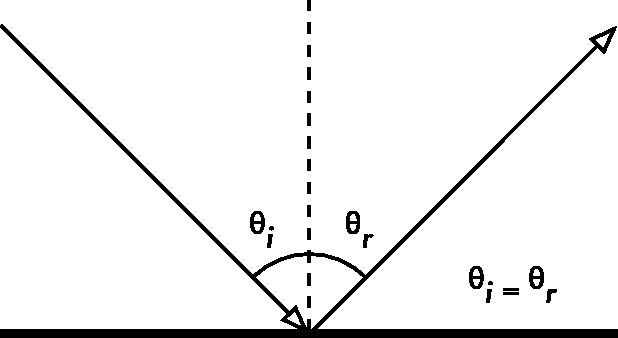
\includegraphics[scale=.72]{figuras/reflexao.pdf}
	}{
		\Fonte{\citeonline[p. ~18]{flickenger2008}.}%
		\Nota{O ângulo de incidência ($\theta_i$) é igual ao ângulo de reflexão ($\theta_r$).}%
	}
\end{figure}

\subsubsection{Multipercurso}
\label{subsec:multipercurso}

Ainda que as regras de reflexão sejam relativamente simples, a situação se torna mais complexa por espalhamento das ondas eletromagnéticas ao chocarem-se contra a superfície das construções e objetos ao redor, como pode ser visto na \autoref{fig:multipath} \cite{haykin2008}.  Esses percursos de propagação múltiplos são conhecidos como multipercurso ou multicaminho. Até mesmo quando existe uma linha de visão direta, o multipercurso ainda ocorre devido às reflexões no solo e nas estruturas próximas a estação móvel \cite{rappaport2009}.

\begin{figure}[H]
	\centering
	\Caption{\label{fig:multipath}Sinais refletidos geram o multipercurso.}	
	\UECEfig{}{
		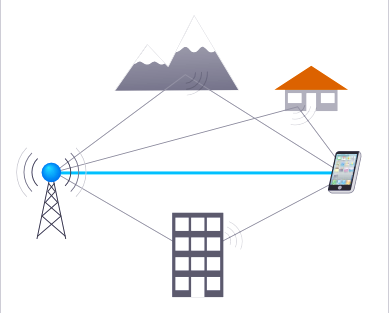
\includegraphics[scale=.8]{figuras/Multipath1.png}
	}{
		\Fonte{Adaptado de \citeonline{yatebts2015}.}
	}
\end{figure}

\subsection{Difração}
\label{sub:difracao}

O fenômeno da difração está relacionado ao fato de as ondas eletromagnéticas contornarem objetos quando passam ao redor dos mesmos, tais como arestas de construções ou picos de montanhas (\autoref{fig:difracao}) ou quando atravessam barreiras contendo aberturas. Para altas frequências, a difração, assim como a reflexão, depende do formato do objeto, além da amplitude, fase e polarização da onda incidente sobre o ponto difrator \cite{rappaport2009}.

\begin{figure}[H]
	\centering
	\Caption{\label{fig:difracao}Difração no topo de uma montanha.}	
	\UECEfig{}{
		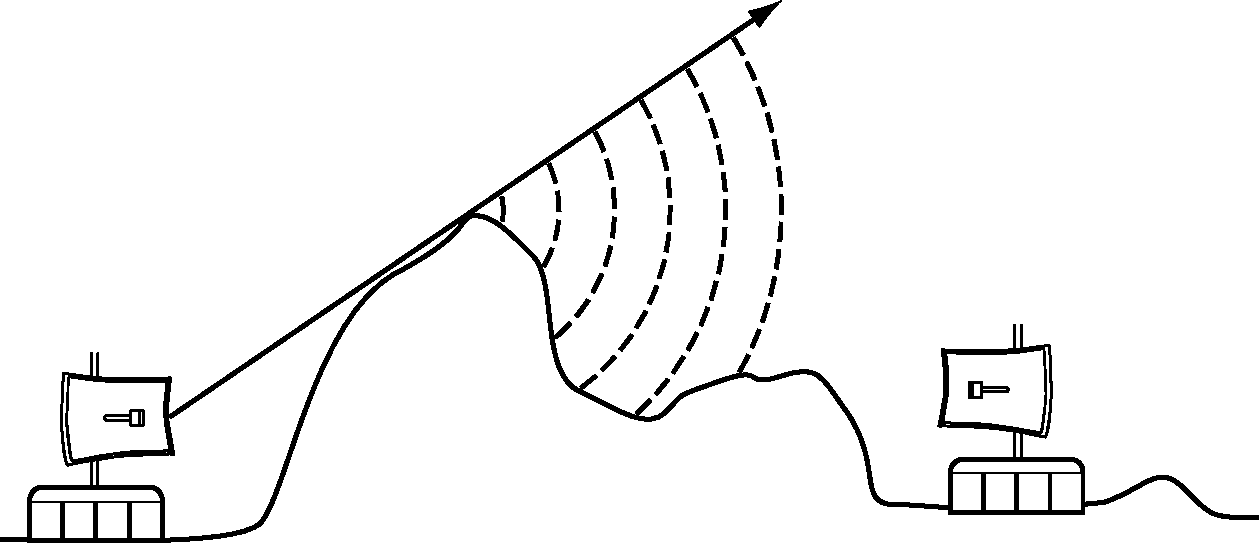
\includegraphics[scale=.6]{figuras/difracao1.pdf}
	}{
		\Fonte{\citeonline[p. ~20]{flickenger2008}.}
	}
\end{figure}

Vale ressaltar que a difração ocorre ao custo de perda de potência, isto é, a energia da onda difratada é significativamente menor que a da onda original. Mas ainda sim existe, nas ondas secundárias resultantes, força suficiente para produzir um sinal útil, além da vantagem da difração para contornar obstáculos entre transmissor e receptor \cite{flickenger2008,rappaport2009}.

\subsection{Refração}
\label{sub:refracao}

A refração ocorre quando as ondas eletromagnéticas mudam a trajetória de propagação quando passam de um meio para outro, assim como mostra a \autoref{fig:refracao}. Na transição, o nível de energia da onda é reduzido, pois uma fração da onda é refletida \cite{flickenger2008}. Um exemplo de refração ocorre quando a luz, propagando-se no ar, encontra uma interface com a água. A utilização da refração nas comunicações sem fio fica limitada a circunstâncias especiais, tais como comunicações via satélite, pois a transmissão necessita penetrar através das camadas da atmosfera, cada uma com densidade distinta da outra \cite{rappaport2009}.

\begin{figure}[H]
	\centering
	\Caption{\label{fig:refracao}Refração.}	
	\UECEfig{}{
		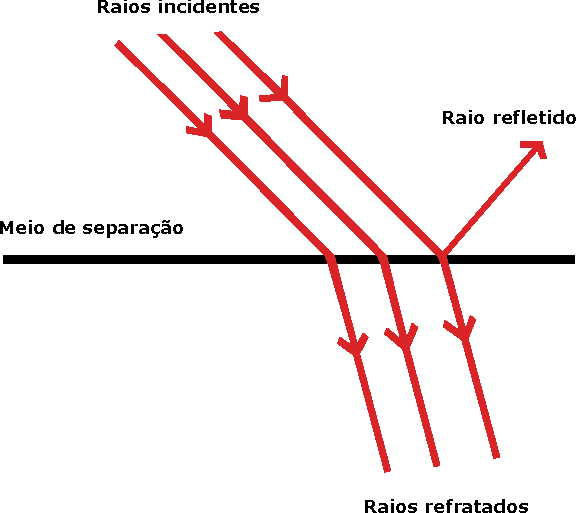
\includegraphics[scale=.69]{figuras/refracao.pdf}
	}{
		\Fonte{Adaptado de \citeonline{teixeira2019c}.}
	}
\end{figure}

\subsection{Interferência}
\label{sub:interferencia}

Interferência é o fenômeno que corrompe um sinal enquanto ele viaja em um enlace da origem para o destino. A perturbação pode interromper, obstruir, degradar ou limitar a recepção efetiva de sinais. Esses efeitos podem variar de uma simples degradação de dados a uma perda total de dados. O termo é frequentemente usado para se referir à adição de sinais indesejados a um sinal útil \cite{flickenger2008}.

Em comunicações sem fio, a interferência é causada principalmente por fontes de radiofrequência que operam na mesma faixa de frequência, como por exemplo, o aparelho de microondas e as redes 802.11 (detalhadas no capítulo 3), ambas operando na banda de 2.4 GHz \cite{moraes2010}. A \autoref{fig:interferencia} mostra um exemplo de interferência entre ondas de rádio.
\begin{figure}[H]
	\centering
	\Caption{\label{fig:interferencia}Interferência entre ondas de rádio.}	
	\UECEfig{}{
		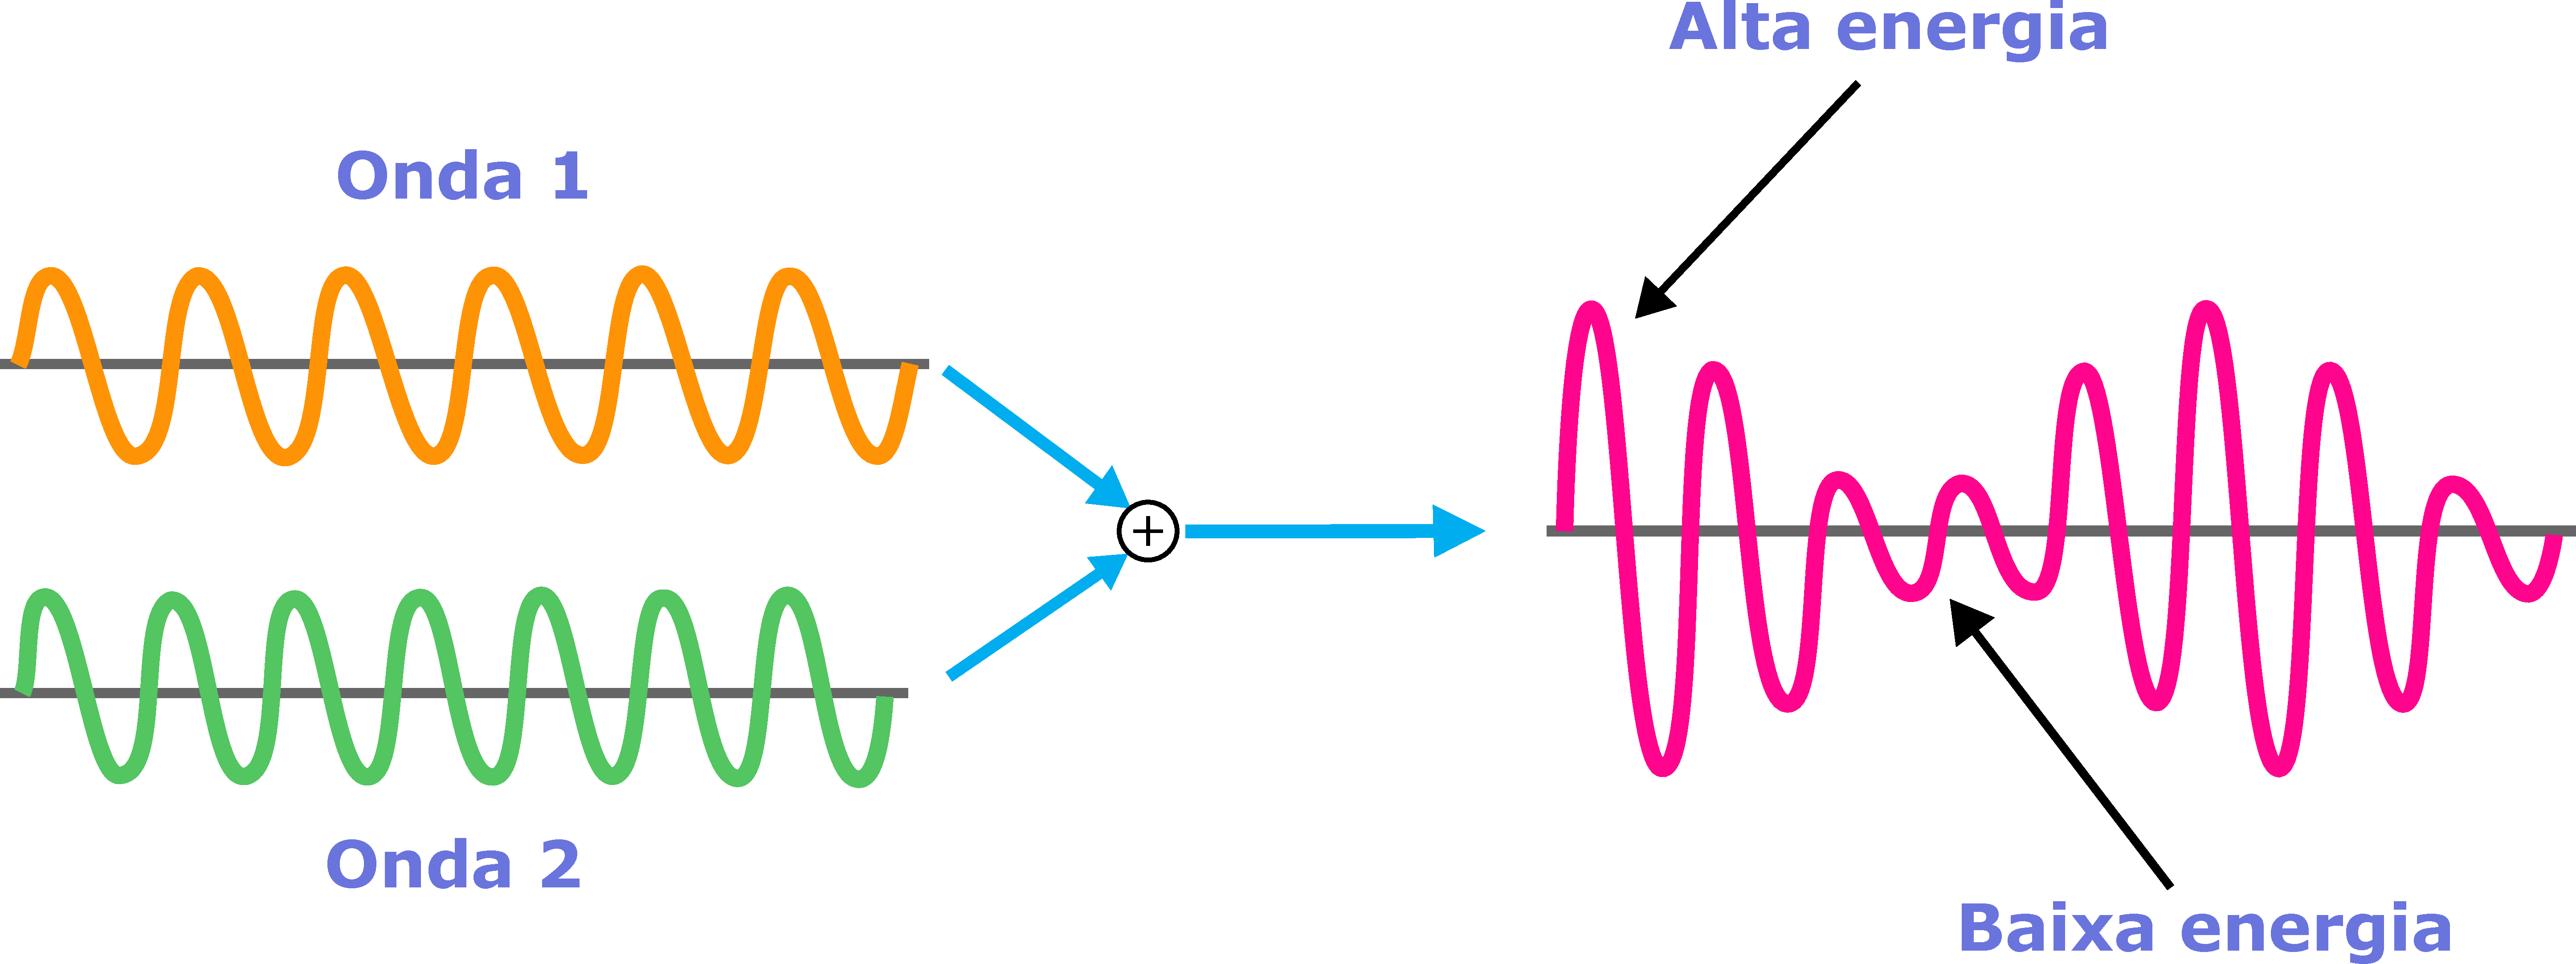
\includegraphics[scale=.13]{figuras/interferenciaSVG_pdf.pdf}
	}{
		\Fonte{Adaptado de \citeonline{physics2015}.}
	}
\end{figure}

\subsection{Desvanecimento (\textit{fading})}
\label{sub:desvanecimento}

O desvanecimento é um fenômeno causado pela variabilidade da intensidade do sinal no tempo associado à mobilidade da estação móvel \cite{haykin2008,rappaport2009}. Frequentemente, o sinal recebido é uma combinação de vários modos de propagação resultantes da reflexão e da difração. Assim, a maior parte da comunicação acontece por espalhamento das ondas eletromagnéticas, que chegam de diferentes direções com diferentes atrasos de propagação \cite{haykin2008}. No receptor, o sinal final é a soma vetorial dessas ondas de caminhos múltiplos, podendo interagir umas com as outras construtiva ou destrutivamente (\autoref{fig:fading}), dependendo da amplitude e da fase de cada componente espectral \cite{haykin2008}.

\begin{figure}[H]
	\centering
	\Caption{\label{fig:fading}Interferência construtiva e destrutiva.}	
	\UECEfig{}{
		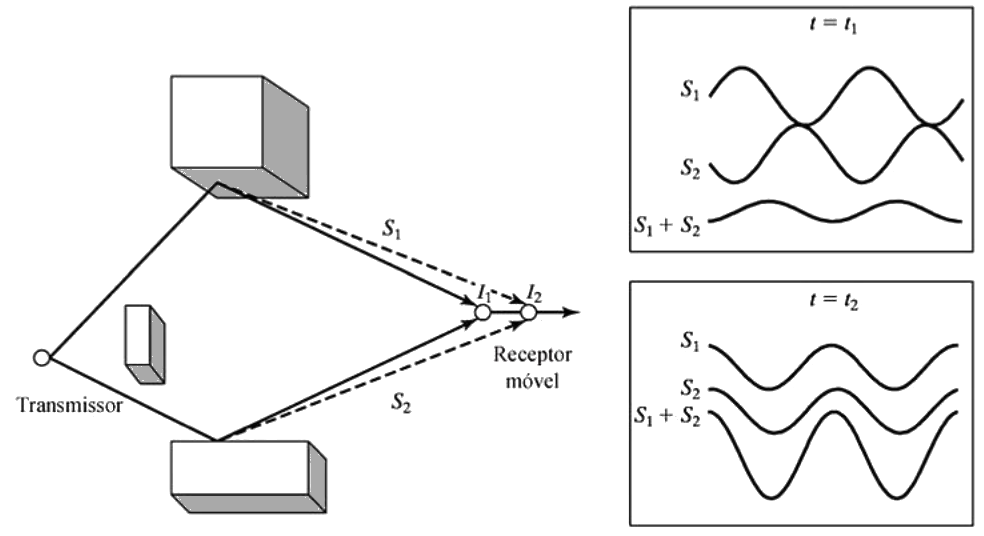
\includegraphics[scale=.35]{figuras/inter.png}
	}{
		\Fonte{\citeonline[p. ~57]{haykin2008}}
	}
\end{figure}

A rapidez com que as flutuações na intensidade do sinal ocorre pode ser classificada como desvanecimento lento (\textit{slow-fading}) ou desvanecimento rápido (\textit{fast-fading}), como ilustra a \autoref{fig:fading-slow-fast} \cite{haykin2008}.

O desvanecimento lento origina-se devido ao efeito da mobilidade do terminal do usuário. É o resultado de mudança de caminho (reflexões) de sinal devido a obstruções como árvores ou edifícios distantes do receptor. O movimento relativo da estação móvel em relação a esses objetos é pequeno, o que resulta em uma perda de percurso pequena \cite{haykin2008}.

O desvanecimento rápido surge devido a alternância nos modos de interferência construtiva e destrutiva causados por multipercurso, juntamente com a velocidade de deslocamento do terminal em relação aos objetos refletores e difratores \cite{haykin2008}.

\begin{figure}[H]
	\centering
	\Caption{\label{fig:fading-slow-fast}Desvanecimento lento e desvanecimento rápido.}	
	\UECEfig{}{
		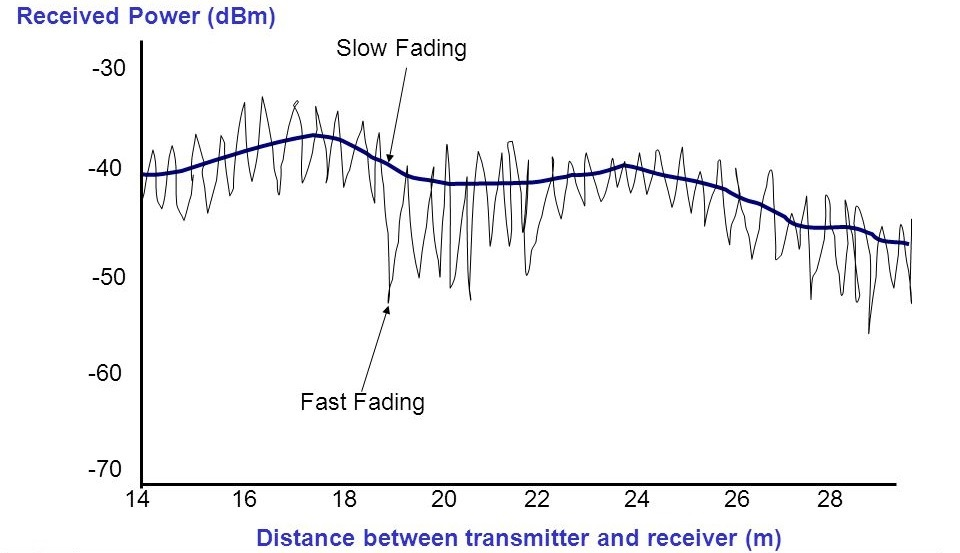
\includegraphics[scale=.5]{figuras/Slow-Fast-Fading.jpg}
	}{
		\Fonte{\citeonline{akkaya2019}.}
	}
\end{figure}

\section{Modelos de Propagação}
\label{sec:modelos-propagacao}

Para que se possa realizar um projeto de enlace de rádio confiável e com boa eficiência, são utilizados os chamados modelos de propagação. Os mesmos são desenvolvidos com base em medições empíricas que buscam alimentar com dados todo um processo matemático complexo capaz de representar a proliferação das ondas de rádio, predizer a perda de caminho ou a cobertura efetiva de um transmissor \cite{akpaida2018,najnudel2004}. Assim, é fácil concluir que, quanto mais informações for possível representar nestas equações, mais precisa será a caracterização do meio e seus efeitos \cite{akpaida2018}.

Modelos de propagação de rádio são empíricos por natureza. E como todos os modelos empíricos, os modelos de propagação de rádio não chamam a atenção para a conduta exata de uma conexão, mas sim para prever o comportamento que o \textit{link} pode mostrar sob as condições especificadas \cite{akpaida2018}.

Existem diversos modelos de propagação formulados por estudiosos e organizações voltadas para o ramo das comunicações sem fio. Cada modelo aplica-se a uma determinada situação específica, dependendo da característica física do local (região urbana ou região rural, por exemplo); frequência de operação do sistema de comunicação e o tipo de material da construção, fator este, crítico para as redes Wi-Fi.

\subsection{Modelo de propagação no espaço livre}
\label{sub:espaco-livre}

O modelo de propagação no espaço livre é usado para prever a intensidade do sinal recebido quando o transmissor e o receptor possuem um linha de visada, ou seja, um caminho livre entre eles \cite{rappaport2009}. Os sistemas de comunicação via satélite normalmente experimentam uma transmissão com caminho desobstruído.

O modelo de espaço livre, assim como a maioria dos modelos de propagação de radiofrequência, prevê que a potência recebida diminui em função da distância de separação transmissor-receptor (T-R) \cite{rappaport2009}. A potência no espaço livre recebida por uma antena receptora que está separada de uma antena transmissora, irradiando, por uma distância T-R é dada pela equação do espaço livre:

\begin{equation}
	\begin{aligned}
	\label{eq:friis}
		P_R = \dfrac{P_TG_TG_R}{L_P}
	\end{aligned}
\end{equation}

\noindent onde $P_T$ é a potência transmitida, $P_R$ é a potência recebida, $G_T$ é o ganho da antena transmissora, $G_R$ é o ganho da antena receptora e $L_P$ é a perda do percurso entre T-R. Tanto a dedução matemática do ganho da antena ($G$) quanto a da perda do percurso ($L_P$) pode ser encontrada com detalhes em \citeonline{haykin2008}.

A Eq. \eqref{eq:friis} é conhecida como equação de Friis. É possível simplificá-la em função do ganho em decibel (dB) \cite{haykin2008}:
\begin{equation}
	\begin{aligned}
	\label{eq:friis-decibel}
		P_R(dB) = P_T(dB) + G_T(dB) + G_R(dB) - L_P(dB)
	\end{aligned}
\end{equation}

\noindent onde $X(dB) = 10\log_{10} (X)$. A equação de Friis é a equação fundamental para o planejamento do enlace de rádio, pois relaciona as potências transmitida e recebida, considerando as condições da transmissão \cite{haykin2008}. Ela fornece os requisitos essenciais para que o nível de potência requerida pelo receptor seja suficiente para ele detectar as informações que lhe foram transmitidas com confiabilidade \cite{haykin2008}.

\subsection{Modelo de dois raios}
\label{sub:modelo-2-raios}

A equação do espaço livre (Eq. \eqref{eq:friis}) considera que sempre existe uma linha de visada direta entre transmissor e receptor, não considera, entretanto, o efeito da superfície terrestre na comunicação. Esse fato raramente acontece com transmissões em solo, o que torna o modelo de espaço livre impreciso na grande maioria dos casos \cite{rappaport2009}.

O modelo de reflexão no solo, baseado na ótica geométrica, considera o caminho direto e um caminho de propagação refletido no solo entre o transmissor e o receptor, como ilustra a \autoref{fig:2raios} \cite{rappaport2009}.

\begin{figure}[H]
	\centering
	\Caption{\label{fig:2raios}Modelo de reflexão no solo com dois raios.}	
	\UECEfig{}{
		%\fbox{\begin{varwidth}{\dimexpr\textwidth-2\fboxsep-2\fboxrule\relax}
		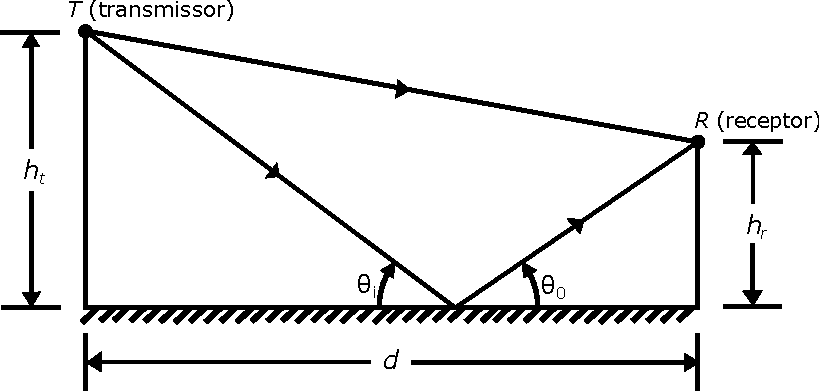
\includegraphics[scale=.4]{figuras/modelo2raios.pdf}
		%\end{varwidth}}
	}{
		\Fonte{Adaptado de \citeonline[p. ~80]{rappaport2009}}
	}
\end{figure}

A potência recebida a uma distância $d$ do transmissor para o modelo de dois raios pode ser expressa como \cite{rappaport2009}:
\begin{equation}
	\begin{aligned}
	\label{eq:2-raios}
		P_R = P_TG_TG_R\dfrac{h^2_Th^2_R}{d^4}
	\end{aligned}
\end{equation}

\noindent onde $h_T$ é a altura do transmissor e $h_R$ é a altura do receptor. Todo o desenvolvimento algébrico até chegar a Eq. \eqref{eq:2-raios} pode ser encontrada em \citeonline{rappaport2009} ou \citeonline{haykin2008}.

\subsection{Modelo log-distância (log simplificado)}
\label{sub:log-distancia}

Os modelos de propagação baseados em medições em campo indicam que que a potência média do sinal recebida cai logaritmicamente com a distância, seja em enlaces de rádio para ambientes fechados (\textit{indoor}) ou abertos (\textit{outdoor}) \cite{rappaport2009}. A perda de percurso média para a uma separação T-R qualquer é obtida em função da distância usando um expoente de perda de caminho, $n$, dada por
\begin{equation}
	\begin{aligned}
	\label{eq:log-distancia}
		PL(d) \propto \left(\dfrac{d}{d_0}\right)^n
	\end{aligned}
\end{equation}

\noindent ou

\begin{equation}
	\begin{aligned}
	\label{eq:log-distancia-2}
		PL(dB) = PL(d_0) + 10n\log_{10}\left(\dfrac{d}{d_0}\right)^n
	\end{aligned}
\end{equation}

\noindent onde $PL$ é a perda média do percurso, $n$ é o expoente de perda de caminho (indica a velocidade com a qual essa perda aumenta com relação a distância), $d_0$ é a distância de referência próxima que é determinada pelas medições perto do transmissor, e $d$ é a distância de separação T-R. O valor de $n$ é calculado usando-se a equação de Friis (modelo de espaço livre) ou por medições de campo à distância $d_0$. A Tabela 1 lista os expoentes típicos de perda de percurso em diversos ambientes.

\begin{table}[H]
	\Caption{\label{tab:tabela-perda-de-percusso}Expoentes de perda de percurso ($n$) para diferentes ambientes.}%
	\IBGEtab{}{%
		\begin{tabular}{lc}
			\toprule
			\multicolumn{1}{c}{Ambiente} & \multicolumn{1}{c}{Expoente de perda de percurso ($n$)} \\
			\toprule %\midrule
			Espaço livre & 2 \\
			
			Rádio-celular em área urbana & 2,7 a 3,5 \\
			
			Rádio-celular urbano sombreado & 3 a 5 \\
			
			Na linha de visão do prédio & 1,6 a 1,8 \\
			
			Obstruído no prédio & 4 a 6 \\
			
			Obstruído em prédio & 2 a 3 \\
			\bottomrule
		\end{tabular}%
	}{%
		\Fonte{\citeonline[p.~91]{rappaport2009}.}%
		%\citeonline[p. ~465]{lott2001ieee}; \apudonline[p.~73]{lott2001ieee}{geier2002}
	}%
\end{table}

\subsection{Modelo de Okumura--Hata}
\label{sub:okumura-hata}

O modelo de Okumura-Hata baseia-se em medições puramente empíricas voltadas especificamente para a predição de sinal de redes celulares para diferentes ambientes. A melhor aplicação do modelo de Okumura-Hata acontece na faixa de frequência existente entre 150 MHz e 1 GHz, podendo ser estendido até 1,5 GHz \cite{haykin2008,rappaport2009}. 

Os dados originais foram medidos por Okumura (entre outros) em diversos locais do Japão. Algum tempo depois, Hata forneceu a equação para predição da perda de propagação em área urbana, juntamente com outras equações de correção para aplicações em área suburbana e aberta.

As perdas do percurso, em dB, para esses três tipos de meios, respectivamente, são dadas pelas equações
\begin{equation}
\begin{split}
	\label{eq:okumura-hata}
		L_P & = A + B\log_{10}r \\
		L_P & = A + B\log_{10}r - C \\
		L_P & = A + B\log_{10}r - D
\end{split}
\end{equation}

\noindent onde $r$ é o alcance em quilômetros, os parâmetros $A$, $B$, $C$ e $D$\footnote[2]{As equações que permitem determinar os valores de $A$, $B$, $C$ e $D$ fogem ao escopo deste trabalho e, por isso, podem ser encontrados na literatura em \citeonline{haykin2008}.} dependem da frequência de operação ($f_c$), da altura da estação transmissora ($h_T$) e da altura da estação receptora ($h_R$).

\subsection{Modelo Multi--Wall--and--Floor}
\label{sub:modelo-MWF}

O modelo \emph{Multi-Wall-and-Floor} (MWF) leva em consideração a perda decrescente de penetração de paredes/pisos da mesma categoria, à medida que o número de paredes/pisos atravessados aumenta, isto é, defende que a relação entre as  perdas não segue uma linearidade lógica \cite{lott2001ieee}. Por exemplo, dada uma perda de penetração de 2 dB em uma parede de concreto, essa mesma onda, ao penetrar em outra parede de mesma característica, não sofrerá uma atenuação de 2 dB como ocorrido no primeiro obstáculo.

O modelo MWF, proposto por \citeonline{lott2001ieee}, é voltado especialmente para a análise dos efeitos da propagação em ambientes \textit{indoor}, pois esses locais concentram grande variedade de divisórias construídas com diferentes materiais. A perda sofrida por uma onda de rádio ao atravessar múltiplas paredes/pisos, $L_{P}$, pode ser dada pela seguinte equação:
\begin{equation}
	\begin{aligned}
	\label{eq:mwf}
		L_{P} = L_0 + 10n\log_{10}(d) + \sum_{i=1}^{I} \sum_{k=1}^{K_{wi}} L_{wik} + \sum_{j=1}^{J} \sum_{k=1}^{K_{fj}} L_{fjk}
	\end{aligned}
\end{equation}

\noindent onde $L_0$ é a perda de trajetória a uma distância de 1m, $n$ é o fator de perda do percurso, $d$ é a distância entre o transmissor e o receptor, $L_{wik}$ é a atenuação devido ao tipo de parede $i$ e à $k$-ésima parede atravessada, $L_{fjk}$ é a atenuação devida ao tipo de piso $j$ e ao $k$-ésimo piso atravessado, $I$ é o número de tipos de parede, $J$ é o número de tipos de piso, $K_{wi}$ é o número de paredes atravessadas do tipo $i$ e $K_{fj}$ é o número de paredes atravessadas do tipo $j$. 

O valor da perda de penetração varia de acordo com o tipo de material ao qual o obstáculo foi construído. A \autoref{tab:tabela-mwf} lista alguns valores de perda de penetração para diversos tipos de material para medições feitas na faixa de frequência de 5.8 GHz.
\newpage
\begin{table}[H]
	\Caption{\label{tab:tabela-mwf}Valores de perda de penetração da parede para o modelo MWF para 5.8 GHz.}%
	\IBGEtab{}{%
		\begin{tabular}{lcc}
			\toprule
			\multicolumn{1}{c}{Material da parede} & \multicolumn{1}{c}{Espessura} & \multicolumn{1}{c}{$k=1$} \\
			\toprule %\midrule
			Madeira compensada & 0.4 cm & $L_{w1I} = 0.9\ dB$ \\
			
			Parede de gesso (rebocada com 1mm de gesso) & 13.5 cm & $L_{w2I} = 3.0\ dB$ \\
			
			Aglomerado de madeira & 1.5 cm & $L_{w3I} = 1.0\ dB$ \\
			
			Vidro plano &  & $L_{w4I} = 2.5\ dB$ \\
			
			Janela de vidro duplo (com uma camada de ar de 12mm) & 2.0 cm & $L_{w5I} = 12\ dB$ \\
			
			Parede de bloco de concreto armado & 30.2 cm & $L_{w6I} = 10\ dB$ \\
			\bottomrule
		\end{tabular}%
	}{%
		\Fonte{Adaptado de \apudonline[p. ~467]{lott2001ieee}{ERC1999}.}%
	}
\end{table}
